\chapter{Синтез алгоритма буфера компенсации джиттера прибытия пакетов на основе робастного фильтра Калмана} \label{chapt3}

\section{Синтез математической модели процесса задержки} \label{sect3_1}
Перед синтезом алгоритма буфера компенсации джиттера необходимо определится с моделью задержки. Достаточно конструктивной моделью случайного динамического процесса, является формирующий фильтр, описываемый уравнением состояния.

\begin{equation}\label{eq3:modelStatDif}
dx(t)/dt=\Phi(t)x(t)+G(t)\xi(t).
\end{equation}

Учитывая то, что мы рассматриваем информационный обмен в цифровой форме в виде пакетов, уравнение состояния, описывающее случайные изменения задержки на каждом из$k$ шагов дискретизации, представляется в виде:

\begin{equation}\label{eq3:modelStat}
x(k+1)=\Phi(k+1,k)x(k)+G(k)\xi(k),
\end{equation}

\noindent где $\Phi(k+1,k)$ - матрица перехода; $G(k)$ - порождающий коэффициент; $\xi(k)$ - порождающая последовательность выборки из гауссовского белого шума (ГБШ), со спектральной плотностью мощности $N_\xi$.

Процесс измерения задержки будем считать линейным. Уравнение наблюдения в линейном приближении представляется в виде:
\begin{equation}\label{eq3:Estim}
y(k)=Hx(k)+\nu(k),
\end{equation}

\noindent где $\nu(k)$ - фазовый шум ошибки измерения, являющийся порождающей последовательностью выборки из гауссовского белого шума со спектральной плотностью мощности $N_\nu$, некоррелированный с процессом $\xi(k)$. 
Как показывают многочисленные исследования в статистике, модель описанная уравнением (\ref{eq3:modelStat}), является идеализированной, в реальных же ситуациях процесс задержки претерпевает различные случайные скачки и выбросы, обусловленные наличием инерционных элементов, таких как буферы, маршрутизаторы и др.

Как мы видим из раздела \ref{chapt2}, процесс задержки имеет различные возмущения, вызванные различными причинами и, следовательно, математическая модель задержки должна учитывать все эти возмущения.
Очевидно, указанные выбросы и скачки задержки можно представить, как уравнение состояния (\ref{eq3:modelStat}) так и как уравнение наблюдения (\ref{eq3:Estim}). Учитывая то, что указанные выбросы является, как правило, ложными и алгоритм буфера должен учитывать их амплитуду в полной мере то, логичнее ввести выбросы в уравнение наблюдения. И наоборот, учитывая то, что алгоритму буфера необходимо как можно раньше определить скачек задержки и переключиться на новый уровень, логичнее ввести скачки задержки в уравнение состояния.

При наличии кратковременных выбросов компонента помех $\xi(k)$ соответственно преобразовывается, с учетом вероятности появления выброса $r_v(k)$. Данная компонента приобретает вид:

\begin{equation}\label{eq3:v}
\xi(k)=(1-r_v(k))\xi(k)+r_v(k)\xi_v(k)
\end{equation}

\noindent где $\xi_v(k)$ представляет собой случайный процесс выброса, а $r_v(k)$ представляет собой последовательностью случайных величин с двумя значениями на каждом шаге: «нуль» или «единица». Вероятности появления этих значений $P(r_v=0)=p_0$ и $P(r_v=1)=p_1$ определяют долю засоренности стационарного случайного процесса $\xi(k)$ выбросами. Когда $r_v=0$ - случайный процесс  $\xi(k)$ имеем нормальный отсчет, а когда $r_v=1$ - имеет аномальный выброс.

Иная ситуация при появлении скачка, который влияет на уравнение состояния в целом, после скачка в уравнение наблюдения появляется смещение, изменяющее несколько последующих состояний, это уравнение представлено в виде:

\begin{equation}\label{eq3:s}
x(k)=(1-r_s(k))x(k)+r_s(k)x_s(k)
\end{equation}

\noindent где $x_s(k)$ представляет собой уравнение состояния случайного процесса скачка, а $r_s(k)$ представляет собой последовательностью случайных величин с двумя значениями на каждом шаге: «нуль» или «единица». Вероятности появления этих значений определяют долю засоренности скачками уравнения состояния. 
Учитывая то, что в рассматриваемой модели имеет место два типа уравнения состояния: для выброса и для скачка, необходимо дополнительное устройство, предназначенное для идентификации типа изменений, которое будет рассмотрено дальше.
С помощью предложенной модели случайного процесса сгенерируем ряд задержек с выбросами на рис. \ref{img3:modelJitter} a) и ряд задержек со скачками задержки на рис. \ref{img3:modelJitter} б).

\begin{figure} [h]
\begin{minipage}[h]{0.47\linewidth}
\center
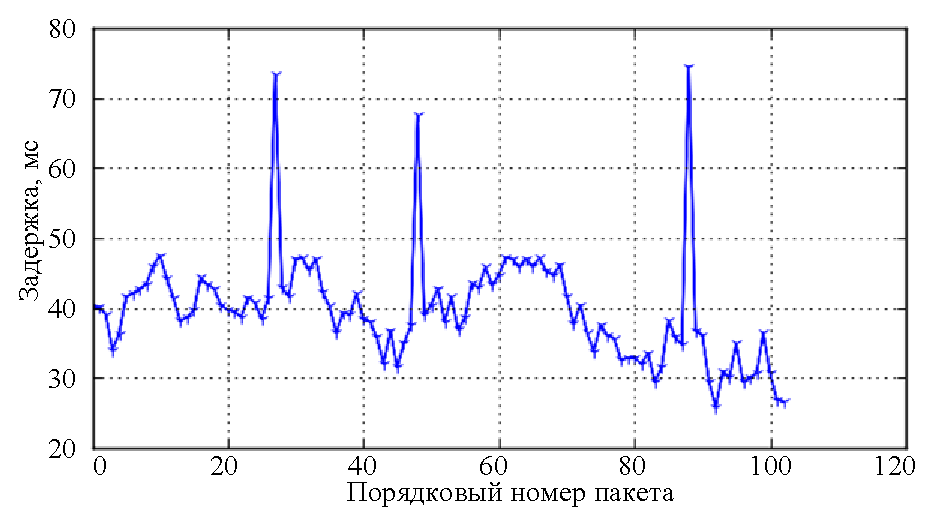
\includegraphics[width=1\linewidth , height=4.5cm]{3chapter/3_1_a.eps} а) \\
\end{minipage}
\hfill
\begin{minipage}[h]{0.47\linewidth}
\center
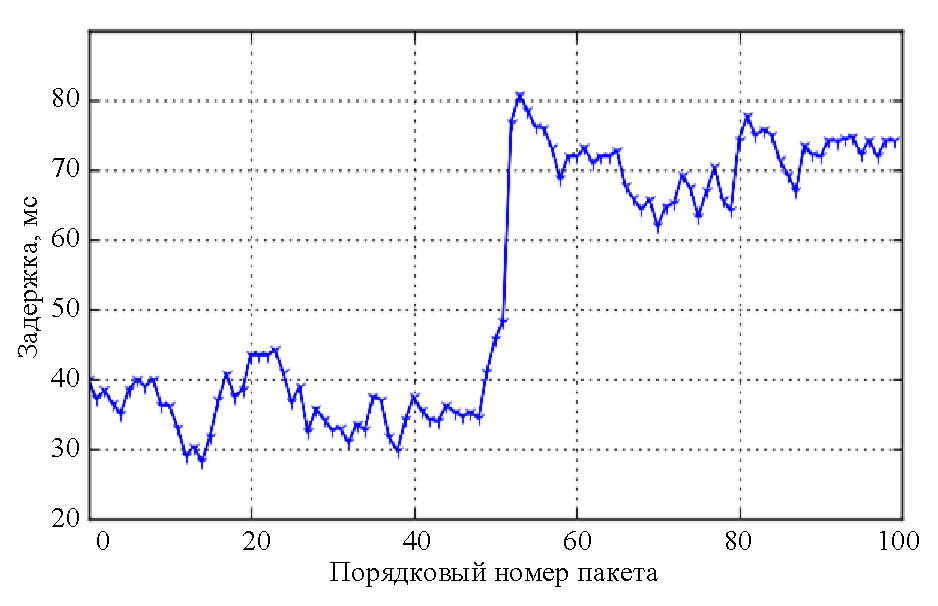
\includegraphics[width=1\linewidth, height=4.5cm]{3chapter/3_1_b.eps} б) \\
\end{minipage}
\caption{Моделирование ряда задержек a) с выбросами, б) со скачками}
\label{img3:modelJitter}
\end{figure}

В результате была получена математическая модель изменения задержки, которая будет использоваться в дальнейшем для моделирования буфера компенсации джиттера.

\section{Обзор принципа работы буфера компенсации джиттера и рабочих характеристик применительно к передаче потокового трафика через IP сети} \label{sect3_2}

Буфер воспроизведения в приемнике удерживает каждый принятый пакет на величину времени буфера, в котором компенсируется джиттер без чрезмерной задержки воспроизведения. Если межпакетная задержка будет превышать буферное время, буфер будет истощаться, и декодеру не будет хватать пакетов, чтобы воспроизводить речь. Это приводит к неравномерности воспроизведения речи. 
Согласно рекомендации ITU G.1020 \cite{G1020} пакеты, прибывающие к получателю с различными ухудшениями, вызванные терминалом источника, сетью или вообще могут быть потеряны, обрабатываются согласно процессу, изображенному на рис. \ref{img3:algh_pack}.

\begin{figure} [h]
  \center
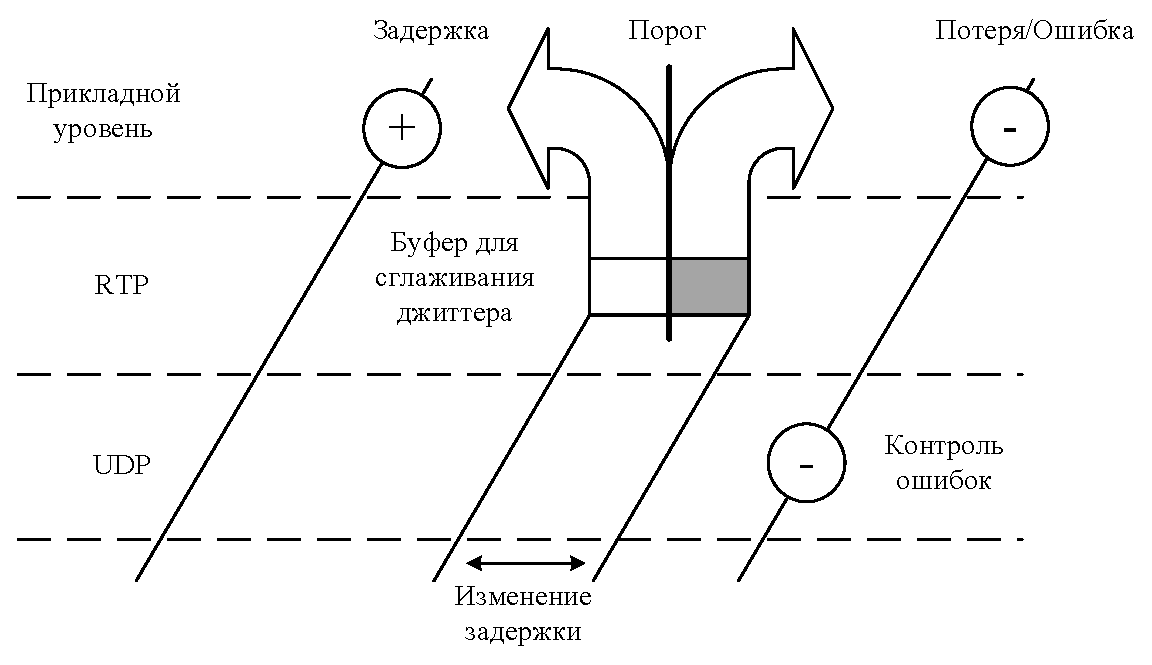
\includegraphics[width=0.95\textwidth]{3chapter/3.eps}
  \caption{Алгоритм обработки сетевых пакетов}
  \label{img3:algh_pack}
\end{figure}

Прибывающие пакеты обрабатываются по мере их продвижения по стеку протокола, для того чтобы удалить как можно больше ухудшений. Показано, что некоторые виды ухудшений, такие как ошибки и джиттер преобразуются в другие ухудшения, такие как общие потери и общие ошибки.
На рис. 3.7 показан компромисс между задержкой и потерями, представленные в виде порока в диапазоне изменения задержки, основанном на размере буфера для сглаживания джиттера. Пакеты с задержкой находящейся в белой зоне будут приняты, тогда как пакеты с задержкой находящейся в черной зоне будут отброшены. Ясно, что чем дольше задержка, тем больше пакетов прибудет до их времени воспроизведения и тем лучше будет компенсация джиттера. В тоже время, длительные задержки нежелательны, так как они ухудшают интерактивность человеческого общения. Отметим, что человеческое ухо терпимо относится к максимальным задержкам от 150 до 400 миллисекунд \cite{Moon}. Различные схемы кодирования также могут иметь различные допуски к потерям. Как следствие, хороший алгоритм компенсации джиттера должен быть в состоянии найти компромисс между задержкой воспроизведения и потерями пакетов.
Рассмотрим изменение процесса потерь во время взаимодействие пакетов с буфером компенсации джиттера. В зависимости от критерия, определяющего решение принимать или отбрасывать каждый конкретный пакет из потока, в результате может полностью измениться распределение общих потерь и общей задержки. Например, если случайные битовые ошибки вызывают ошибки в контрольной сумме UDP, то потери пакетов будут иметь случайное распределение, по мере того как они поступают на прикладной уровень. Но, если несколько последовательных пакетов испытывают чрезмерные задержки, то дополнительные отбрасывания, вызванные ограничениями буфера компенсации джиттера, сделают общее распределение потерь скорее прерывистым, чем случайным.
Существуют обстоятельства, при которых порядок следования пакетов может изменяться во время их прохождения через сеть. Некоторые буферы компенсации джиттера неспособны восстановить порядок следования переупорядоченных пакетов и, в этом случае, они обозначаются как отброшенные пакеты.
Также рассмотрим влияние буфера компенсации джиттера на процесс задержки. На рис. \ref{img3:delNode} показаны основные элементы речевого тракта, которые вносят вклад в речевую задержку. Задержка сети переменна и для компенсации джиттера и восстановления допустимого интервала между пакетами используют буфер компенсации джиттера. Заметим, что пакеты с минимальной задержкой на стороне отправителя и сети, проводят максимальное время в буфере компенсации джиттера; и наоборот, пакеты, которые задерживаются дольше минимального времени, проводят затем в данном буфере меньшее время. Кроме того, существует еще, и некоторое минимальное количество времени, которое каждый пакет должен проводить в буфере на стороне получателя, которое может быть столь же велико, как и целый пакет.

\begin{figure} [h]
  \center
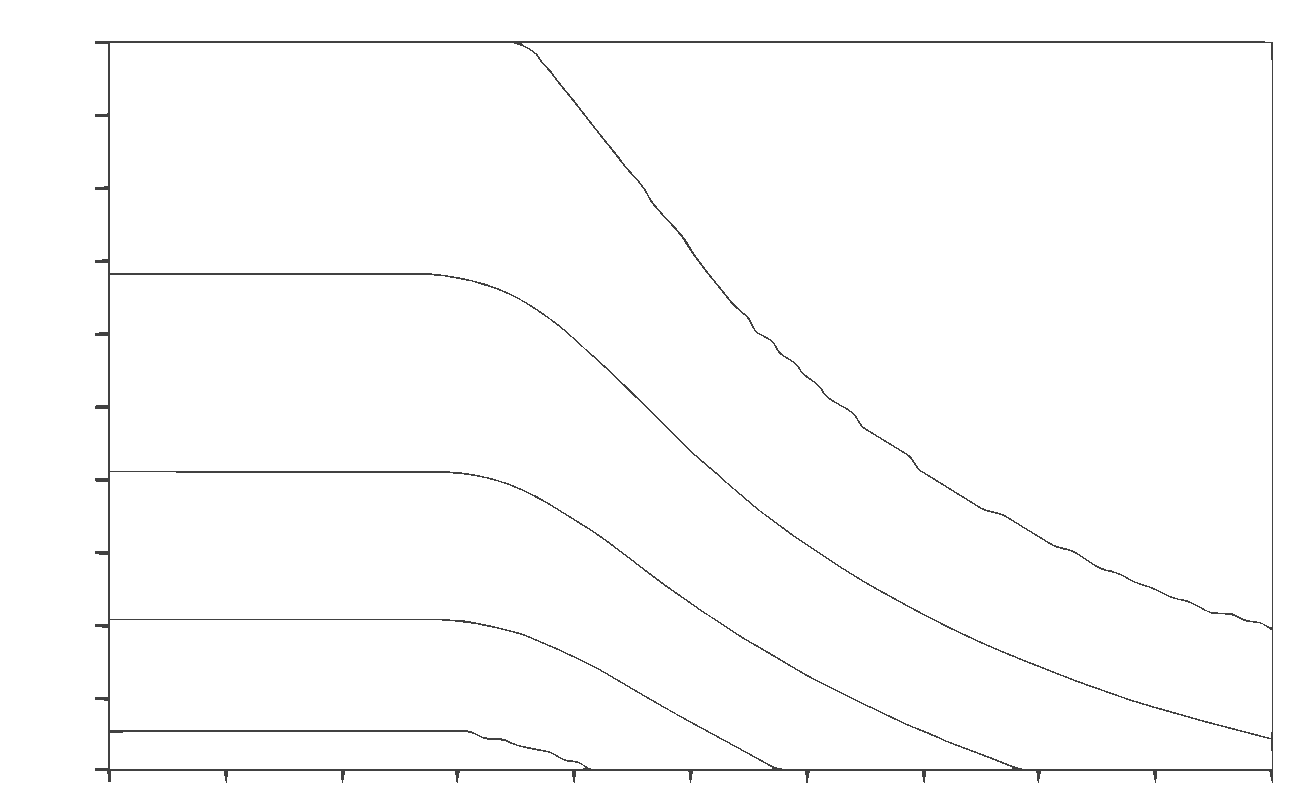
\includegraphics[width=0.95\textwidth]{3chapter/2.eps}
  \caption{Задержка в пакетных сетях и сетевых элементах}
  \label{img3:delNode}
\end{figure}

Правильное значение задержки буфера для объединения с другими задержками зависит от наличия описательной статистики. Например, среднюю задержку в сети следует суммировать со средним временем использования буфера компенсации джиттера, чтобы получить общую среднюю задержку. Этот метод предусматривает адаптацию буфера, требуя знания только среднего времени пребывания всех пакетов в очереди в оцениваемом временном интервале. С другой стороны, если известна только минимальная задержка в сети, то ее следует суммировать с максимальным временем использования буфера компенсации джиттера, чтобы дать общую задержку.
Далее рассмотрим инициализацию буфера компенсации джиттера фиксированного размера. Если первый прибывающий пакет имеет минимальную задержку передачи, то получатель будет сохранять этот пакет в буфере все необходимое время, и размер буферизации будет равен ожидаемому. К счастью, многие пакеты прибывают за время, равное или близкое к минимальному времени передачи, поэтому этот случай весьма правдоподобен. 
С другой стороны, если первый пакет имеет довольно большую задержку, то для размещения ранее принятых пакетов со временем передачи, равным или близким к минимальному времени передачи, потребуется больше буферного пространства, а буфер для сглаживания фазового дрожания будет вносить в общий расчет задержку, превышающую ожидаемую.

\section{Систематизация типов, параметров и моделей буферов компенсации джиттера} \label{sect3_3}

Существуют два основных типа буферов компенсации джиттера – фиксированной длины и адаптивной длины. Буферы компенсации джиттера, согласно рекомендации \cite{G1020}, могут быть построены с использованием разных способов, приведенных в табл. \ref{TypeBuff}.

\begin{table} [htbp]
  \centering
  \parbox{15cm}{\caption{Типы и параметры буфера компенсации джиттера}\label{TypeBuff}}
\begin{tabular}{|p{3cm}||p{4cm}|p{4cm}|p{4cm}|}
    \hline
    \hline
    Тип                        & Атрибуты                                                            & \multicolumn{2}{|c|}{Возможности}                                                                                                                                                                    \\ \hline \hline
    Фиксированный и адаптивный & Размер (конфигурируется максимальная и номинальная или минимальная) & Целое количество пакетов                                                     & Дробное количество пакетов                                                                                             \\ \hline
\multirow{6}{*}{Адаптивный}    & Управление                                                          & Синхронизированное ослабление при отсутствии переполнения / антипереполнения & Оценить коэффициент потерь (конфигурировать приемлемый наименьший порог и минимальный счет пакетов между подстройками) \\ 
\cline{2-4}
                               & Подстройка                                                          & Синхронизированная                                                           & Только в промежутках молчания                                                                                          \\
\cline{2-4}
                               & Инициализация                                                       & Первый пакет                                                                 & Малая выборка                                                                                                          \\ 
\cline{2-4}
                               & Неравномерность подстройки                                          & Размер пакета                                                                & Дробная часть пакета                                                                                                   \\ 
\cline{2-4}
                               & Восстановление порядка пакетов                                      & Да                                                                           & Нет                                                                                                                    \\ 
\cline{2-4}
                               & Режим передачи данных в полосе тональных частот                     & Обнаружение тональной частоты 2100 Гц; установка максимальной длины          & Нет                                                                                                                    \\ 
\hline
    \end{tabular}
\end{table}


Более подробно рассмотрим параметры построения алгоритма адаптивного буфера компенсации джиттера по методу подстройки задержки воспроизведения, такие как алгоритмы выполняющие коррекцию синхронно и алгоритмы выполняющие коррекцию в промежутках между речевыми потоками. 
В схеме с синхронизированной подстройкой задержки воспроизведения (рис. \ref{img3:manageDelay} a)) время воспроизведения всех последующих пакетов растягивается всякий раз, когда пакет чрезмерно задерживается в сети. 
Во втором случае, показанном на рис. \ref{img3:manageDelay} б), производится корректировка первого пакета речевого потока, а все остальные пакеты воспроизводятся через фиксированный интервал после первого пакета. Пакеты, прибывшие позже, отбрасываются, и кодек может либо повторить последний принятый пакет или вставить паузу или поиграть другие экстраполированные звуки.


\begin{figure} [h]
\begin{minipage}[h]{0.85\linewidth}
\center
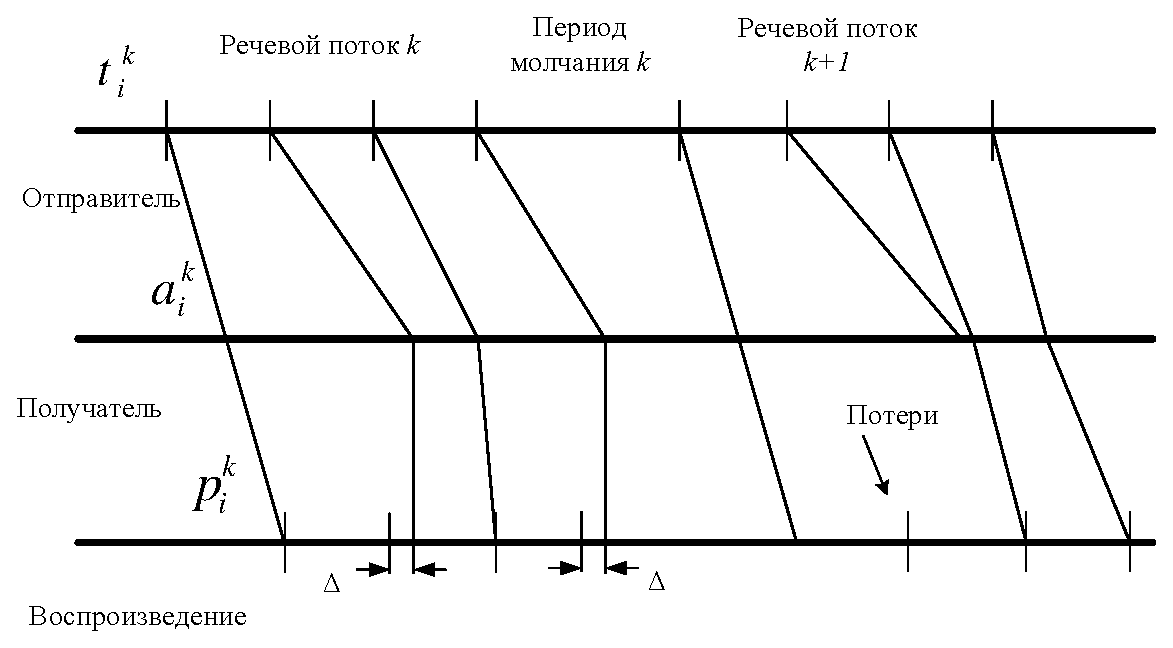
\includegraphics[width=1\linewidth]{3chapter/4a.eps} а) \\
\end{minipage}
\vfill
\begin{minipage}[h]{0.95\linewidth}
\center
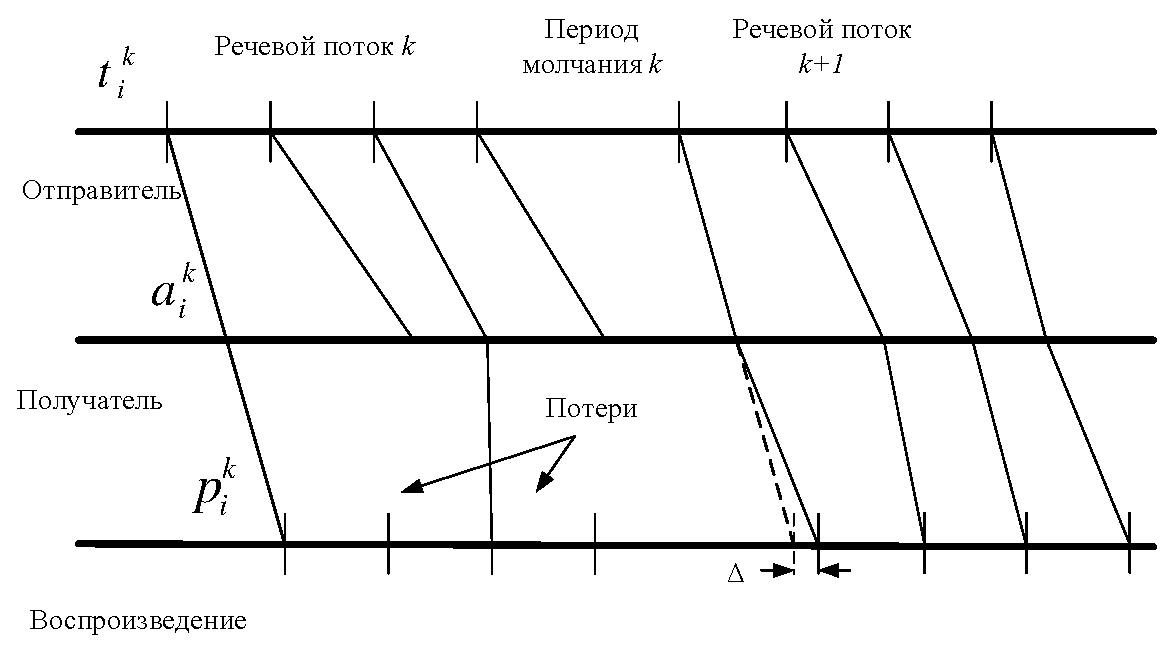
\includegraphics[width=1\linewidth]{3chapter/4b.eps} б) \\
\end{minipage}
\caption{Схема регулировки задержки воспроизведения в паузах между речевыми потоками а) с синхронной подстройкой б) с подстройкой первого пакета речевого потока }
\label{img3:manageDelay}
\end{figure}


Синхронизированный способ сводит к минимуму потери пакетов, но влияет на длину исходного речевого потока, что приводит к проблемам с разборчивостью восстановленной речи. По этой причине разрабатываемый буфер компенсации джиттера будет основан на алгоритме с подстройкой задержки только в периоды молчания.


\section{Анализ существующих алгоритмов компенсации джиттера.} \label{sect3_4}
\subsection{Модель фиксированного буфера компенсации джиттера.} \label{sect3_4_1}

Наиболее простой и эффективной моделью отбрасывания пакетов является фиксированный буфер компенсации джиттера, который обозначает, как отбрасываемые, все пакеты, задержка которых больше чем минимальная задержка передачи потока пакетов плюс фиксированная длина буфера для сглаживания джиттера.
Рассмотрим пример алгоритма от сетевого до прикладного уровня, предполагая что на терминале получателя используется буфер компенсации джиттера с фиксированной длиной:
\begin{enumerate}
\item Отметить как потерянные все пакеты с неверной контрольной суммой UDP.
\item Отметить как отбрасываемые все пакеты, задержка которых больше, чем минимальная задержка передачи потока пакетов плюс (фиксированная) длина буфера для сглаживания джиттера, или задержка которых меньше чем установленный минимум. 
\item Суммировать среднюю задержку в сети со средней задержкой терминала источника и терминала получателя, чтобы получить общую среднюю задержку, или суммировать минимальную задержку в терминале источника и минимальную задержку в сети с максимальной задержкой терминала получателя (отражающую максимальное время использования буфера для сглаживания джиттера).
\end{enumerate}

В вышеприведенном шаге 2 минимальную задержку передачи следует оценивать на коротких интервалах, например 10 секунд. Данное минимальное значение первого интервала используется всегда, не считая краткосрочного увеличения минимума вне диапазона адаптации буфера. В этом случае ни один из пакетов не будет доставлен на верхние уровни и буфер компенсации джиттера должен быть переустановлен на новый минимум, что вероятно будет происходить на практике. Или же, если краткосрочное значение минимума уменьшиться до величины, при которой высокий процент (временно 50\%) пакетов были бы помечены как потерянные из-за раннего поступления, то буфер компенсации джиттера должен быть переустановлен на новый минимум.

\subsection{Модель адаптивного буфера компенсации джиттера.} \label{sect3_4_2}

Фиксированный буфер компенсации джиттера может быть заменен эмуляцией адаптивного буфера компенсации джиттера, как описано в данном пункте, когда имеется информация о временной последовательности потока пакетов. 
Временные последовательности поступления пакетов могут быть использованы эмулятором адаптивного буфера компенсации джиттера при определении динамики размера буфера и среднего времени использования буфера (задержка) для этой последовательности. Эта средняя задержка может быть объединена с другими константами задержки в терминале получателя для получения оценки средней задержки в терминале получателя. 
Рассмотрим пример эмулятора адаптивного буфера для сглаживания джиттера с коррекцией задержки в промежутках молчания \cite{Ramjee}. Чтобы определить время воспроизведения для пакета $i$-ого, мы рассмотрим два случая, в зависимости от того является $i$-ый пакет первым в речевом потоке или нет:
Если $i$-ый пакет является первым в речевом потоке, то его время воспроизведения рассчитывается как:

\begin{equation}\label{eq3:playout}
p_i=t_i+\hat{d_i}+\gamma\cdot\hat{\nu_i},
\end{equation}

\noindent где $\hat{d_i}$ и $\hat{\nu_i}$ - это оценка среднего и отклонения сквозной задержки в течении речевого потока, $\gamma$ - это константа, используемая для установки времени воспроизведения так чтобы только небольшая часть поступающих пакетов была потеряна \cite{Ramjee}. Эта константа равна 4 во всех экспериментах, выполняемых в \cite{Ramjee}. В \cite{Moon} это значение варьируют от 1 до 20, что бы добиться различного процента потерь. Чтобы пересчитать среднюю сетевую задержку и его отклонение, используются следующие уравнения:

\begin{equation}\label{eq3:playout_d}
\hat{d}_{i}^{k}=\alpha\cdot\hat{d}_{i-1}^{k}+(1-\alpha)\cdot d_{i}^{k},
\end{equation}

\begin{equation}\label{eq3:playout_v}
\hat{\nu}_{i}^{k}=\alpha\cdot\hat{\nu}_{i-1}^{k}+(1-\alpha)\cdot | \hat{d}_{i}^{k}-d_{i}^{k} |.
\end{equation}

Эти уравнения представляю собой линейные рекурсивные фильтры, где коэффициент $\alpha$ называется шаговой постоянной, $\alpha\leq1$ и обеспечивает устойчивость процедуры. В работе \cite{Ramjee} значение $\alpha$ выбрано равным 0.98002. 

Очевидно, что эти уравнения являются преобразованными уравнениями стохастической аппроксимации типа Роббинса-Монро. Можно показать, что получаемая оценка $\hat{d}_{i}^{k}$ и $\hat{\nu}_{i}^{k}$, является оптимальной для оценивания случайной величины для которых уравнение состояния $x_k=x_{k-1}$. В нашем случае сетевая задержка представляет случайный процесс, для которой оптимальной является процедура Калмана-Бьюси из-за оптимизационной постановки задачи.

\section{Синтез алгоритма буфера компенсатора джиттера на основе фильтра Калмана (ФК)} \label{sect3_5}

Поскольку задержка в соответствии с уравнением (\ref{eq3:Estim}) наблюдается на фоне гауссового белого шума, а само значение задержки случайно из-за множества факторов формирующих эту случайность, то можно утверждать, что в силу центральной предельной теоремы распределение случайной задержки также подчиняется нормальному закону. Знание закона распределения и использование в таких случаях минимума среднеквадратичного отклонения позволяет рассчитывать на то, что полученные оценки окажутся более точными из-за оптимизационной постановки задачи. 
Уравнение оценки в виде условного среднего значения задержки с использованием ФК имеет вид:

\begin{equation}\label{eq3:Estim_rel}
\hat{x}_{k+1}=\Phi\hat{x}(k)+K(k)\Delta y,
\end{equation}
\noindent где $\Delta y=H\Phi\hat{x}(k)-y(k)$ - невязка, $K(k)$ - коэффициент, обеспечивающий устойчивость и сходимость процедуры, в частности $K(k)$ может быть константой $K\leq1$. Коэффициент усиления ФК $K(k)$ является функцией от апостериорной дисперсии ошибки оценки $V(k)$, что ускоряет его сходимость:

\begin{equation}\label{eq3:K}
K(k)=V(k)H^TN_{\nu}^{-1},
\end{equation}
 
\begin{equation}\label{eq3:V}
V(k)=[I-K(k-1)H(k)]V(k,k-1),
\end{equation}


\begin{equation}\label{eq3:Vkk-1}
V(k,k-1)=\Phi^TV(k-1)\Phi+N_\xi,
\end{equation}

\noindent где $V(k)$ - апостериорная дисперсия ошибки оценки, $V(k,k-1)$ - априорная дисперсия ошибки оценки, $I$ - единичная матрица.

На рис. \ref{img3:kalmanF} представлена схема сглаживающего фильтра, построенная в соответствии с (\ref{eq3:Estim_rel}). Ключевую роль в оценке ФК текущего значения задержки, является параметр $\Phi$ позволяющий регулировать сглаживающие свойства фильтра. 

\begin{figure} [h]
  \center
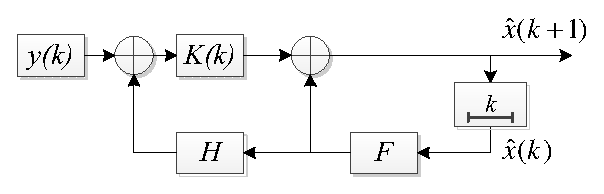
\includegraphics[width=0.6\textwidth]{3chapter/10.eps}
  \caption{Схема ФК}
  \label{img3:kalmanF}
\end{figure}




\subsection{Робастный фильтр Калмана (РФК) для ситуации выброса} \label{sect3_5_1}
Очевидно, что с использованием модернизированного уравнения наблюдения, ФК становится не оптимальным, а его сходимость к установившемуся состоянию проблематичной. Существует несколько методов, позволяющих обеспечить сходимость ФК среди которых метод кусочно-линейной аппроксимации, метод дискретно-непрерывных моделей и др. \cite{Chernavskiy,Rasina}. Данные методы являются близкими к оптимальным, но вычислительно сложны в реализации, поэтому рассмотрим робастный фильтр Калмана (РФК), который является более простым и обеспечивает запас устойчивости в широком диапазоне входных воздействий.
Воспользуемся методологией работы \cite{RobustFilter}. Короткий выброс задержки в уравнении (\ref{eq3:v}) и возвращение ее в стационарное состояние, является, как правило, ложным и основной задачей фильтра, является сгладить данный выброс, обеспечив текущую величину этого значения неизменной по сравнению с прошлым шагом. Процедура Калмана-Бьюси при этом приобретает следующий вид:

\begin{equation}\label{eq3:skachok}
\hat{x}(k+1)=\Phi(k+1,k)\hat{x}(k)+K(k)\Delta y\cdot min\left\{1,\frac{b}{|K(k)\Delta y|}\right\},
\end{equation}

\noindent где $b$ является некоторым ограничителем изменения значения функции. Это предложение убирает проблему неограниченого изменения оценки за один шаг в классическом фильтре Калмана, оставаясь при этом достаточно простой.

Если $b\geq |K(k) \Delta y |$, то $min\left\{1,\frac{b}{|K(k)\Delta y|}\right\}$ и фильтр работает в обычном режиме как ФК (\ref{eq3:Estim_rel}). Если же $b\leq |K(k) \Delta y |$, то из этого следует, что произошел выброс и невязка умножается на понижающий коэффициент, равный $\frac{b}{|K(k)\Delta y|}$, что опять же приводит РФК к обычному виду (\ref{eq3:Estim_rel}).

\subsection{Робастный фильтр Калмана для ситуации скачка} \label{sect3_5_2}

Следуя рекомендации \cite{RobustFilter} РФК для ситуации скачка приобретает вид:

\begin{equation}\label{eq3:vibros}
\hat{x}(k+1)=\Phi(k+1,k)\hat{x}(k)+H(k)[I-H(k)K(k)\Delta y] min\left\{1,\frac{b}{|I-H(k)K(k)\Delta y|}\right\},
\end{equation}

\noindent где $b$ тот же аргумент, ограничивающий изменение значения функции, что и для РФК для ситуации выброса (\ref{eq3:skachok}).

\subsection{Гибридный робастный фильтр Калмана (ГРФК)} \label{sect3_5_3}

Очевидно, одновременная фильтрация возможна только с некоторой задержкой $\Delta \tau$. Это необходимо для принятия решения о типе выброса. Вследствие выброса скорей всего увидим один большой выброс (\ref{eq3:v}), а вследствие скачка – подряд целую последовательность (\ref{eq3:s}). ГРФК может быть реализован следующим образом \cite{RobustFilter}: РФК для ситуации скачка работает по умолчанию и всякий раз, когда ширина выброса больше окна наблюдения $\Delta \tau$, единожды используется процедура РФК для ситуации скачка.


\section{Моделирование оценивания с помощью робастного фильтра случайного процесса с выбросами и скачками} \label{sect3_6}
Чтобы сравнить алгоритмы фильтрации проведем моделирование оценки случайного процесса с помощью приведенных робастных алгоритмов фильтрации и фильтра Калмана. Результаты приведены на рис. \ref{img3:filterIdeal}-\ref{img3:filterMix}. Сплошной линией со снежинками показан наблюдаемый процесс, сплошной – оценка ФК, штрихпунктирной с точками – РФК для ситуации с выбросами, штрихпунктирной - РФК для ситуации со скачками и штрихпунктирной со снежинками – ГРФК. На рис. \ref{img3:filterIdeal} представлены результаты оценивания временного процесса без выбросов и скачков (\ref{eq3:Estim}), из графика следует, что рассмотренные робастные алгоритмы, не теряют своей оптимальности по сравнению с ФК, во время оценивания процесса без выбросов и скачков.
На рис. \ref{img3:filterVibros} представлены результаты оценивания временного процесса с выбросами (\ref{eq3:v}), из графика следует, что РФК для ситуации выброса и ГРФК позволяют игнорировать выбросы, что обеспечивает оптимальную оценку процесса.
На рис. \ref{img3:filterSkachok} представлены результаты оценивания временного процесса со скачками (\ref{eq3:v}), из графика следует, что РФК для ситуации скачка и ГРФК позволяют быстро переключиться на новое значение задержки. В то время как РФК для ситуации выброса оказался не в состоянии отслеживать скачки.
В заключение, на рис. \ref{img3:filterMix} представлены результаты оценивания временного процесса со скачками и с выбросами, из графика следует, что, ГРФК позволяет получить оптимальную оценку в смешанной ситуации, в то время как остальные алгоритмы выполняют оценку недопустимо плохо.

\begin{figure} [h]
  \center
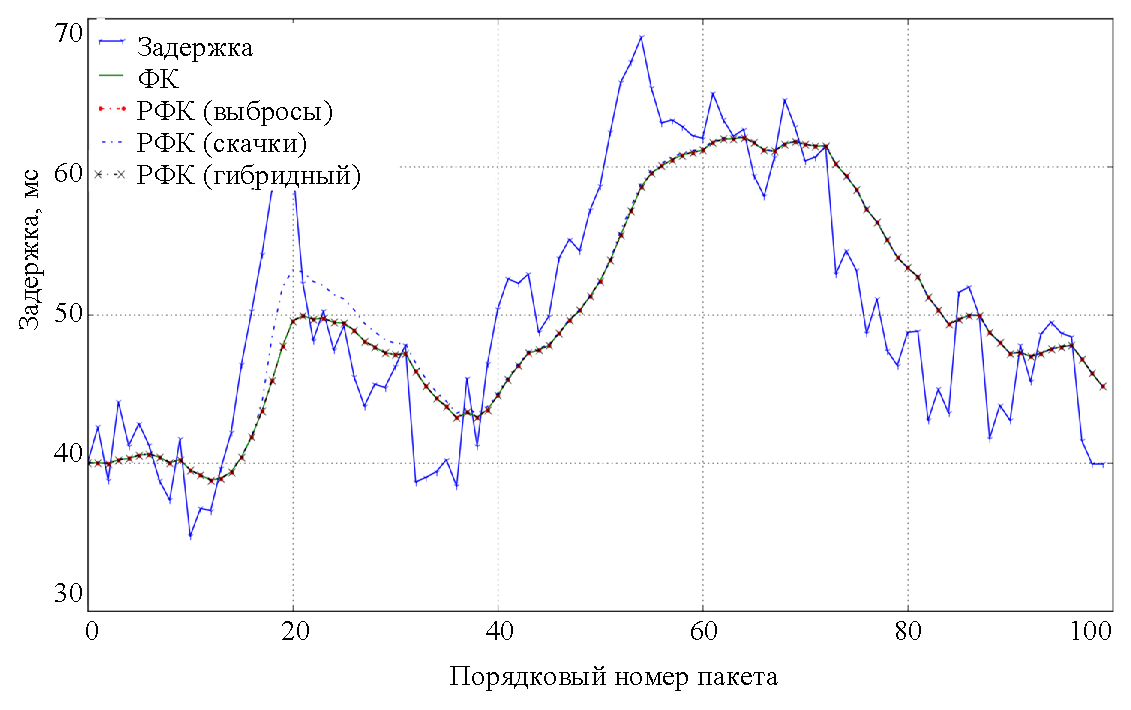
\includegraphics[width=0.95\textwidth]{3chapter/6_1.eps}
  \caption{Моделирование фильтрации в идеальных условиях}
  \label{img3:filterIdeal}
\end{figure}

\begin{figure} [h]
  \center
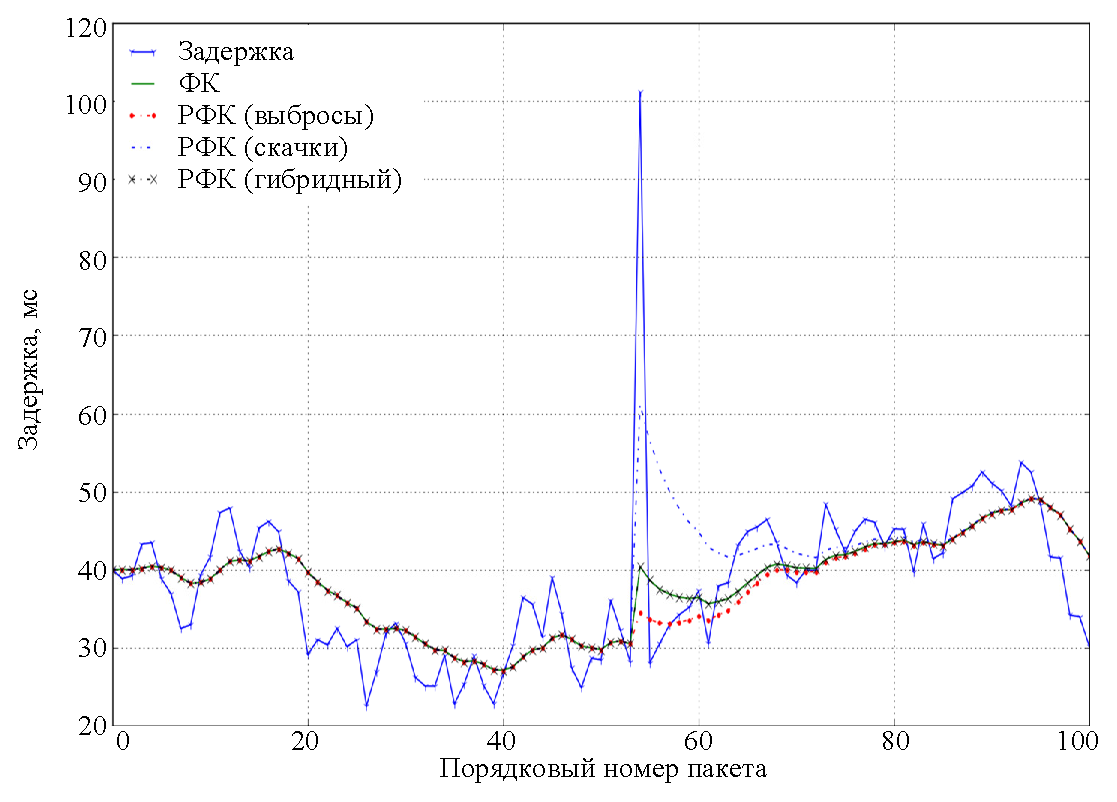
\includegraphics[width=0.95\textwidth]{3chapter/6_2.eps}
  \caption{Моделирование фильтрации при выбросах}
  \label{img3:filterVibros}
\end{figure}

\begin{figure} [h]
  \center
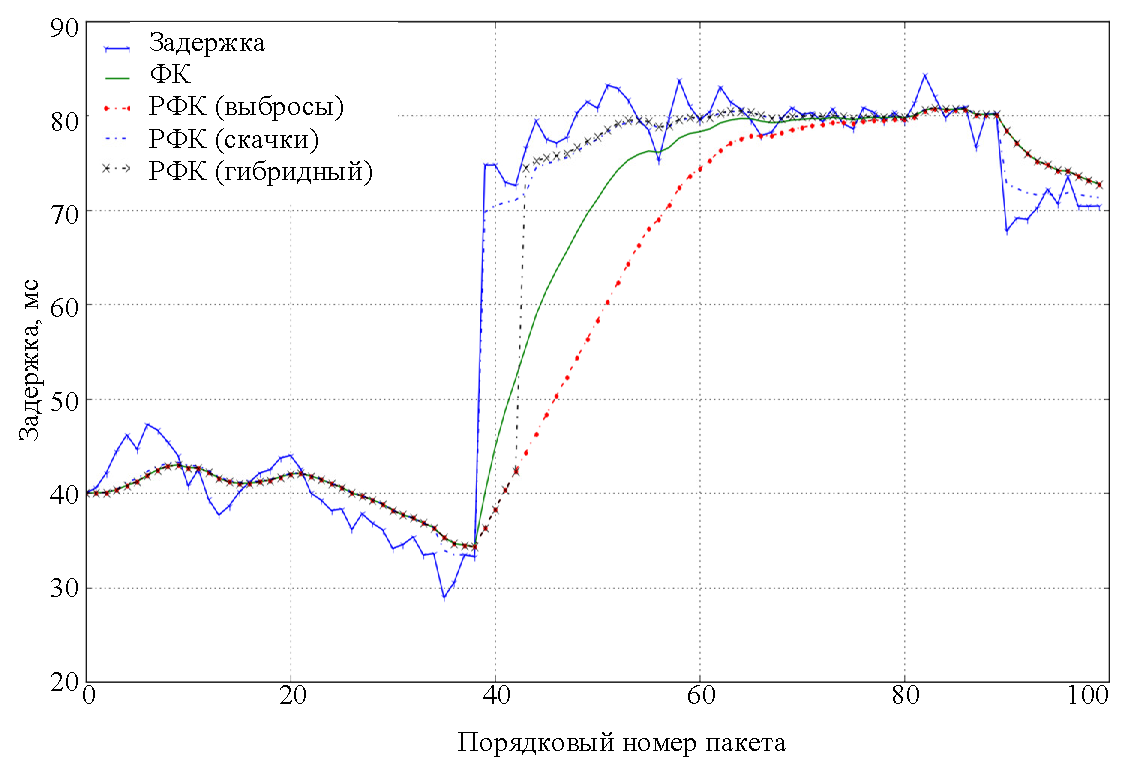
\includegraphics[width=0.95\textwidth]{3chapter/6_3.eps}
  \caption{Моделирование фильтрации при скачках}
  \label{img3:filterSkachok}
\end{figure}

\begin{figure} [h]
  \center
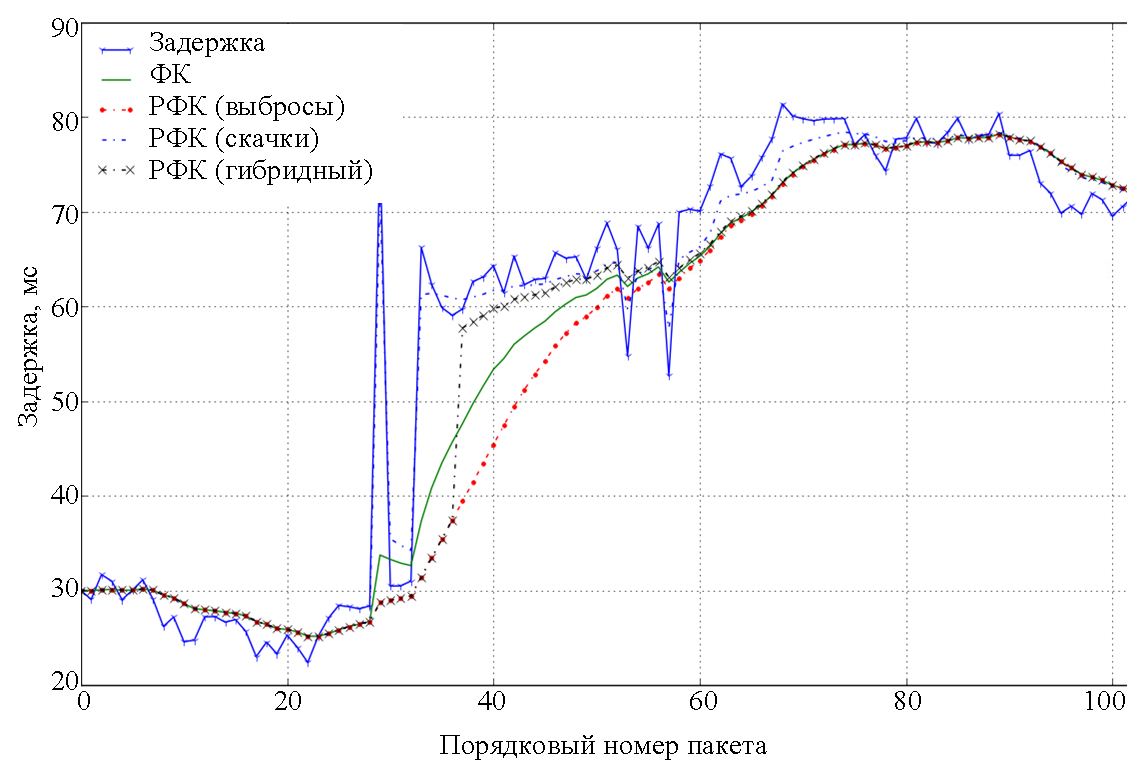
\includegraphics[width=0.95\textwidth]{3chapter/6_4.eps}
  \caption{Моделирование фильтрации в смешанной ситуации скачков и выбросов}
  \label{img3:filterMix}
\end{figure}

В процессе эксперимента был получен средний квадрат отклонений (СКО) оценки в различных ситуациях зашумленности (скачки и выбросы) с помощью рассмотренных фильтров и результаты приведены в табл. \ref{fkDiffSit}



\begin{table} [htbp]
  \centering
  \parbox{15cm}{\caption{Типы и параметры буфера компенсации джиттера}\label{fkDiffSit}}
\begin{tabular}{|p{3cm}|p{3cm}|p{3cm}|p{3cm}|p{3cm}|}
    \hline
    Тип фильтра        & Условия без выбросов и скачков & Условия со скачками & Условия с выбросами & Условия с выбросами и скачками \\ \hline
    ФК                 & 6,48                           & 6                   & \textbf{2,7}                 & 26,6                           \\ \hline
    РФК (для выбросов) & 11,02                          & 29,93               & 3,2                 & 23,1                           \\ \hline
    РФК (для скчков)   & \textbf{2,15}                           & \textbf{0,85}                & 19,8                & 42                             \\ \hline
    ГРФК               & 31,08                          & 10,93               & 27,4                & \textbf{14,4}                           \\ \hline
    \end{tabular}
\end{table}








Жирным шрифтом выделены лучшие результаты оценок по сравнению с другими фильтрами для каждой шумовой ситуации. Как и предполагалось, для ситуации с выбросами и скачками наилучший результат показал гибридный робастный фильтр Калмана.









\clearpage
